\documentclass[tikz,border=4pt]{standalone}
\usepackage[T1]{fontenc}
\usepackage{lmodern}
\renewcommand{\familydefault}{\sfdefault}
\usetikzlibrary{shapes.geometric,positioning,arrows.meta,calc}
\tikzset{
  node distance=6mm,
  every node/.style={font=\footnotesize,align=center,execute at begin node={\hyphenpenalty=10000\relax}},
  base/.style={draw=gray!60,fill=gray!12,minimum height=7mm,inner sep=2pt},
  term/.style={base,rounded corners=3.5mm,text width=30mm},
  proc/.style={base,text width=32mm},
  err/.style={base,text width=30mm,fill=gray!22},
  io/.style={base,trapezium,trapezium left angle=72,trapezium right angle=108,trapezium stretches=true,text width=28mm},
  dec/.style={base,diamond,aspect=2.4,text width=27mm,inner sep=0pt},
  go/.style={-{Stealth[length=2mm]},draw=gray!55!black},
  lab/.style={font=\scriptsize,fill=white,inner sep=1pt},
}

\begin{document}
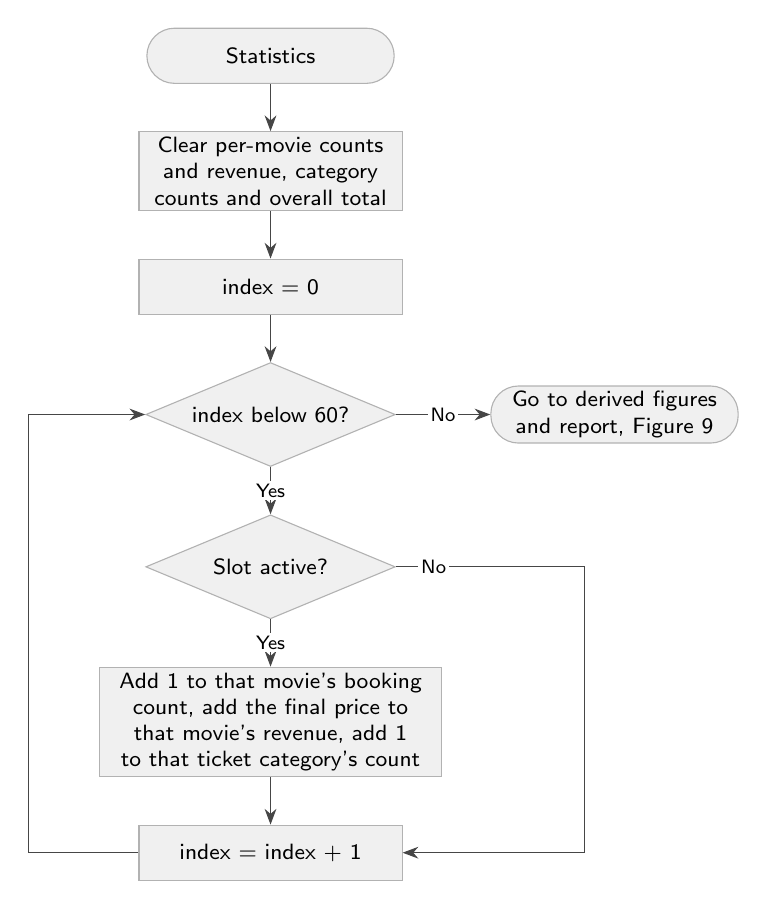
\begin{tikzpicture}
\node[term] (s) {Statistics};
\node[proc,below=of s] (c) {Clear per-movie counts and revenue, category counts and overall total};
\node[proc,below=of c] (i) {index = 0};
\node[dec,below=of i] (d) {index below 60?};
\node[term,right=12mm of d] (g) {Go to derived figures and report, Figure 9};
\node[dec,below=of d] (a) {Slot active?};
\node[proc,below=of a,text width=42mm] (u) {Add 1 to that movie's booking count, add the final price to that movie's revenue, add 1 to that ticket category's count};
\node[proc,below=of u] (n) {index = index + 1};
\draw[go] (s)--(c);\draw[go] (c)--(i);\draw[go] (i)--(d);
\draw[go] (d)--node[lab]{Yes}(a);
\draw[go] (d)--node[lab]{No}(g);
\draw[go] (a)--node[lab]{Yes}(u);
\draw[go] (u)--(n);
\draw[go] (a.east)--node[lab,pos=.2]{No}++(24mm,0)|-(n.east);
\draw[go] (n.west)--++(-14mm,0)|-(d.west);
\end{tikzpicture}
\end{document}
